\documentclass[border=10pt]{standalone}

\usepackage{tikz}
\usepackage{tikzsymbols}
\usetikzlibrary{calc,patterns,shapes.geometric}

\def\centerarc[#1](#2)(#3:#4:#5){\draw[#1] ($(#2)+({#5*cos(#3)},{#5*sin(#3)})$) arc (#3:#4:#5);}

\begin{document}
	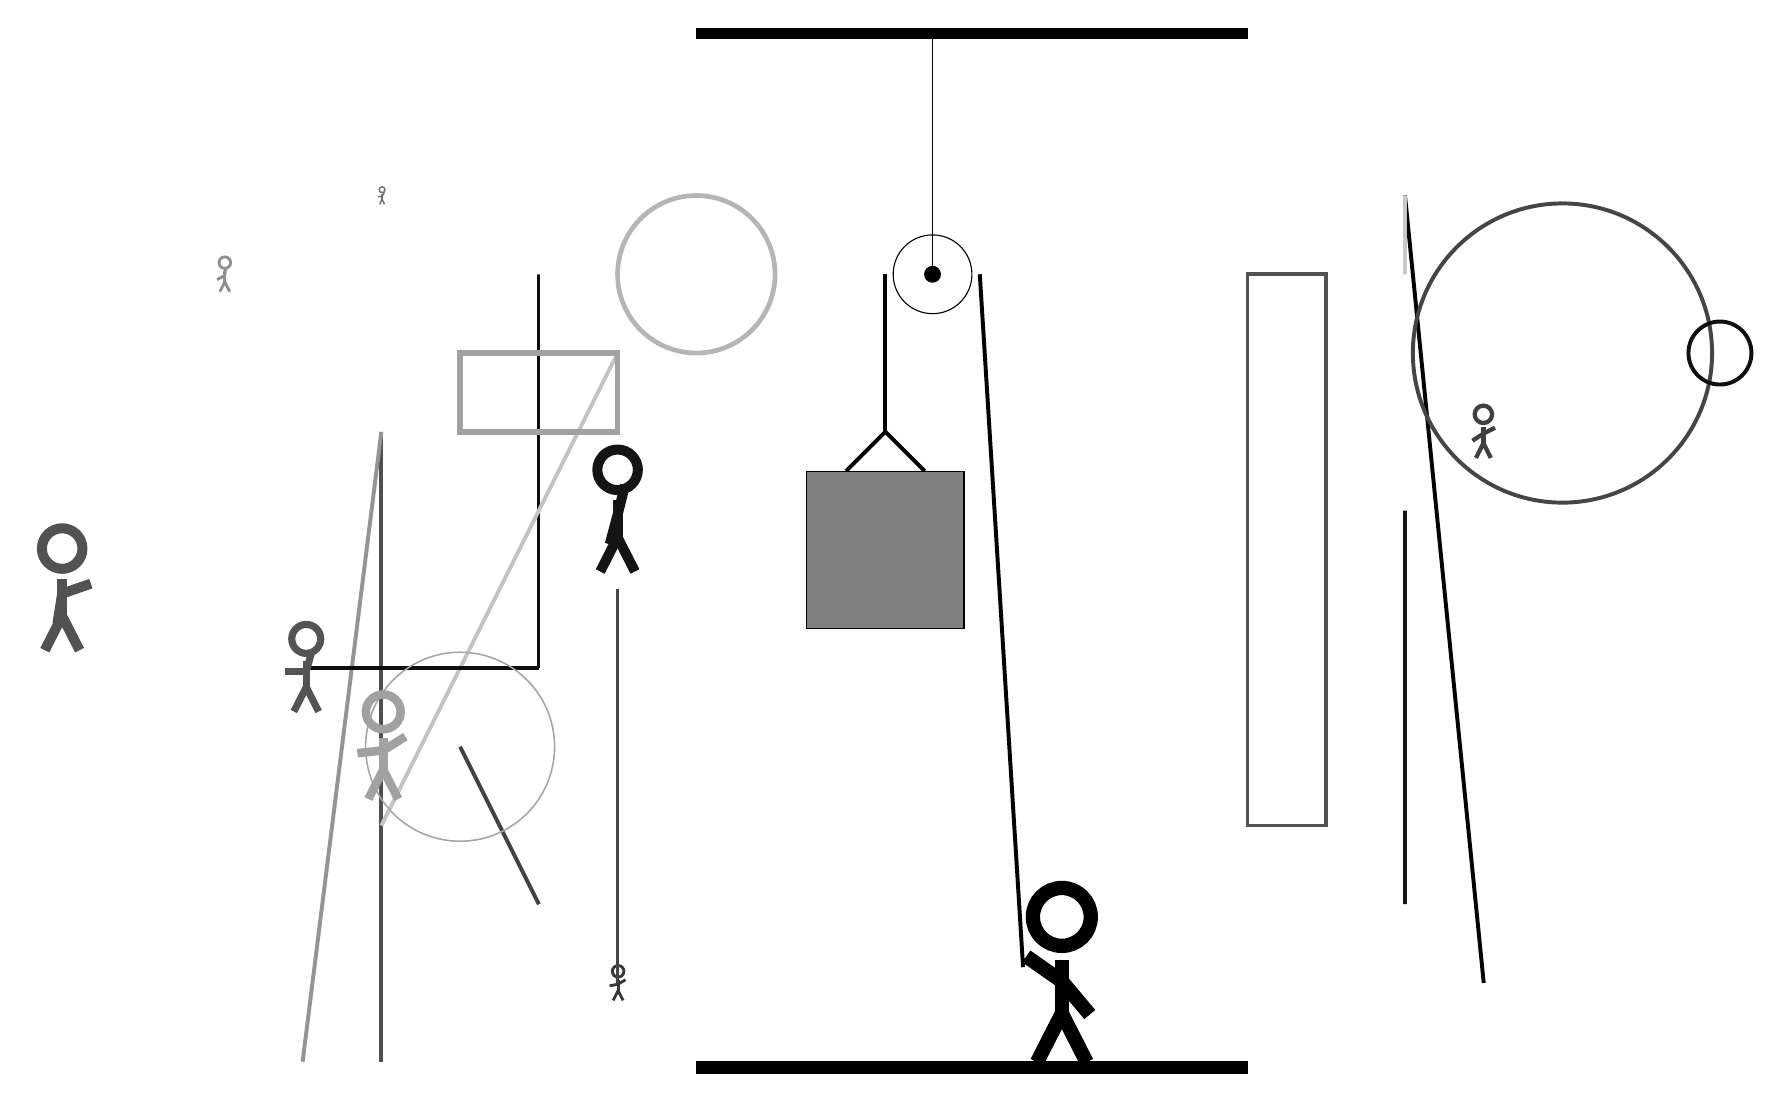
\begin{tikzpicture}
		%%%%% START %%%%%
		
		\draw[fill=black] (-2, 10) rectangle (5, 10.125);
		
		\draw (1, 7) circle (0.5);
		\draw[fill=black] (1, 7) circle (0.1);
		\draw (1, 10) -- (1, 7);
		
		\draw[line width=0.5mm] (-0.1, 4.5) -- (0.4, 5.0) -- (0.9, 4.5);
		\draw[fill=black!50] (-0.6, 4.5) rectangle (1.4, 2.5);
		
		\draw[line width=0.4mm, color=black!95] (-4, 7) rectangle (-4, 2);
		
		\draw[line width=0.5mm, color=black!69](-6, -3) -- (-6, 5);
		\node[line width=0.4mm, color=black!78] at (-3, -2) {\Strichmaxerl[2][11][31]};
		\draw[line width=0.5mm, color=black!74](-4, -1) -- (-5, 1);
		\draw[line width=0.5mm, color=black!23](-3, 6) -- (-6, 0);
		\node[line width=0.4mm, color=black!56] at (-6, 8) {\Strichmaxerl[1][7][56]};
		
		\node[line width=0.5mm, color=black!92] at (-3, 4) {\Strichmaxerl[7][75][76]};
		
		\draw[line width=0.5mm, color=black!42](-7, -3) -- (-6, 5);
		\node[line width=0.7mm, color=black!75] at (8, 5) {\Strichmaxerl[3][33][27]};
		\draw[line width=0.5mm, color=black!95](-4, 2) -- (-7, 2);
		
		\draw[line width=0.5mm, color=black!99](7, 8) -- (8, -2);
		
		\draw [line width=0.6mm, color=black!29](-2, 7) circle (1.0);
		\draw[line width=0.7mm, color=black!37] (-3, 5) rectangle (-5, 6);
		
		\draw[line width=0.5mm, color=black!21] (7, 7) rectangle (7, 8);
		\draw [line width=0.2mm, color=black!35](-5, 1) circle (1.2);
		\draw[line width=0.3mm, color=black!73] (-3, -2) rectangle (-3, 3);
		
		\draw [line width=0.5mm, color=black!73](9, 6) circle (1.9);
		\node[line width=0.6mm, color=black!37] at (-6, 1) {\Strichmaxerl[6][6][32]};
		\draw [line width=0.5mm, color=black!94](11, 6) circle (0.4);
		
		\node[line width=0.4mm, color=black!67] at (-7, 2) {\Strichmaxerl[5][0][74]};
		\draw[line width=0.5mm, color=black!68] (5, 0) rectangle (6, 7);
		
		\node[line width=0.4mm, color=black!68] at (-10, 3) {\Strichmaxerl[7][81][19]};
		\node[line width=0.5mm, color=black!44] at (-8, 7) {\Strichmaxerl[2][28][84]};
		\draw[line width=0.5mm, color=black!92] (7, -1) rectangle (7, 4);
		
		\draw[line width=0.5mm] (0.4, 7) -- (0.4, 5.0);
		\centerarc[line width=0.5mm](1, 7)(0:180:0.6);
		\draw[line width=0.5mm](1.6, 7) -- (2.15, -1.8);
		
		\node at (2.6, -1.9) {\Strichmaxerl[10][-35][-50]};
		
		\draw[fill=black] (-2, -3) rectangle (5, -3.15);
		
		%%%%% END %%%%%
	\end{tikzpicture}
\end{document}